\documentclass[titlepage]{jarticle}
%\usepackage{type1cm}
\usepackage{outline-ec}
\usepackage{amsmath,amssymb,verbatim,ascmac,multicol}
\usepackage{tabularx}
\usepackage{url}
\usepackage[hang,small,bf]{caption}
\usepackage[subrefformat=parens]{subcaption}

%\usepackage{multirow}
% dvioutで確認する場合は以下を有効にする
%\usepackage[dviout]{graphicx,color}
% pdf化する場合は以下を有効にする
\usepackage[dvipdfmx]{graphicx,color}

\captionsetup{compatibility=false}
\captionsetup[subfigure]{labelformat=simple}
\renewcommand{\thesubfigure}{(\alph{subfigure})}
%
% --------------------------------------------------------------------------
% 図表番号の後の:を削除
%
\makeatletter
\long\def\@makecaption#1#2{% #1=図表番号,#2=キャプション本文
  \sbox\@tempboxa{#1 \hskip0.5zw #2}% 図表番号とキャプションの間のスペース 0.5zw
  \ifdim \wd\@tempboxa >\hsize
    #1 #2\par
  \else
    \hb@xt@\hsize{\hfil\box\@tempboxa\hfil}
  \fi}
\makeatother

\氏名{本間 三暉}			%% 自分の氏名
\出席番号{35}					%% 出席番号
\研究室名{視覚情報処理研究室}			%% 研究室名
\指導教官{高橋 章}			%% 指導教員名

\発表番号{B\;--\;1}
\研究題目{単一視点による人物の全身運動の三次元計測について}

\アブストラクト{
慣性式モーションセンサを体表につけた全身運動を行う人物を一台のRGBカメラやRGBDカメラで撮影し,それぞれのカメラに合った画像処理を用いた手法と慣性式モーションキャプチャの座標データでそれぞれ三次元骨格推定を行う.
それぞれの骨格データにキャリブレーションを行い,それぞれのデータを定量的に比較する.
しかし,キャリブレーションの方法が悪かったのか,求めているようなデータが出なかった.
}

\begin{document}
\maketitle

\section{研究背景・目的}
人の動きなどのノンバーバルな情報を,コミュニケーションに用いたりアーカイブすることに活用する目的で,カメラで撮影できる二次元の情報から三次元の情報を推測する技術が求められている.
本研究室では柔道の三次元の動きを複数視点の動画から推測する研究\cite{turugi}が行われている.
しかし,この方法では複数台のカメラの設置やキャリブレーションの手間がある.
また,近年デプスという,カメラと物体までの距離の情報を取得できるカメラが市販されたり,
機械学習を用いることによって単眼カメラから深度推定ができるようになったり,スマートフォンと組み合わせることで手軽に三次元の情報を取得できるようになってきた.

そこで本研究では機械学習を活用して一台の入力装置で三次元骨格推定を行える複数の手法について実装し,
オクルージョンというカメラの手前にある物体に計測する箇所が隠れてしまい,計測の信頼度が下がってしまう状態の有無や,動作の緩急について,それぞれ運動によりの精度を定量的に比較する.
\section{研究内容}
% \subsection{人の動作の計測方法}
%
人の動作の三次元骨格推定を行うには,画像処理による方法やモーションセンサによる方法がある.%それぞれの方法について簡単にまとめたものを表\ref{3D_1}に示す.
% 画像処理による方法では画像から人の骨格を推定することで人の動作を解析できる.
画像処理による三次元骨格推定は撮影するカメラに,色情報を記録できる一般的なRGBカメラを用いる方法
% (\ref{RGB_sec})
と,カメラと物体の距離も取得可能なRGBDカメラを用いる方法
% (\ref{RGBD_sec})
がある(\ref{3Dskeleton}).

モーションセンサによる方法は,光学式や慣性式などがある.
光学式は体表面にマーカーを取り付けそのマーカーを複数台のカメラで取り込むことで骨格を推定する.
慣性式は加速度,角速度,方位を測定できるセンサを体表面の指定箇所に取り付けることで骨格を推定する(\ref{motion}).

%%%あまりにも急展開

本研究では,市販の入力デバイスを使用し,PCで処理可能で複数のカメラで取り込む必要がある光学式モーションキャプチャのような専用の計測空間が不要な3つの方法について性能を比較評価する.
% \begin{table}[t!]
%   \centering
%   \caption{動作を計測する方法の種類と特徴}
%   \begin{tabular}{l|ll|ll}
%     \hline
%                   & \multicolumn{2}{c|}{\small{カメラ}}       & \multicolumn{2}{c}{\small{モーションセンサ}}                                                     \\ \cline{2-5}
%                   & \multicolumn{1}{c|}{\small{RGB}}       & \small{RGBD}                         & \multicolumn{1}{c|}{\small{光学式}} & \small{慣性式}    \\ \hline
%     \small{センサ装着} & \multicolumn{1}{c|}{\small{不要}}        & \small{不要}                           & \multicolumn{1}{c|}{\small{必要}}  & \small{必要}     \\
%     \small{外から撮影} & \multicolumn{1}{c|}{\small{必要}}        & \small{必要}                           & \multicolumn{1}{c|}{\small{必要}}  & \small{不要}     \\
%     \small{必要台数}  & \multicolumn{1}{c|}{\small{1$\sim$数台}} & \small{1台}                           & \multicolumn{1}{c|}{\small{複数台}} & \small{0台}     \\ \hline
%     \small{計測方法}  & \multicolumn{1}{c|}{\small{MediaPipe}} & \small{Nuitrack}                     & \multicolumn{1}{c|}{\small{}}    & \small{mocopi} \\%%%これも怪しいけどね
%     \small{計測関節数} & \multicolumn{1}{c|}{\small{33個}}       & \small{19個}                          & \multicolumn{1}{c|}{\small{}}    & \small{27個}    \\
%     \hline
%   \end{tabular}
%   \label{3D_1}
% \end{table}
\subsection{画像処理による三次元骨格推定}\label{3Dskeleton}
画像処理を用いて三次元骨格推定をしている様子を図\ref{image_3D}に示す.
今回,画像入力装置としてRGBDカメラであるIntel RealSense D415(以下RealSense)を使用する.
カメラの解像度は640$\times$360\,px,フレームレートは60\,fpsとし,実験には明るい室内で撮影を行った.
\begin{figure}[b]
  \centering
  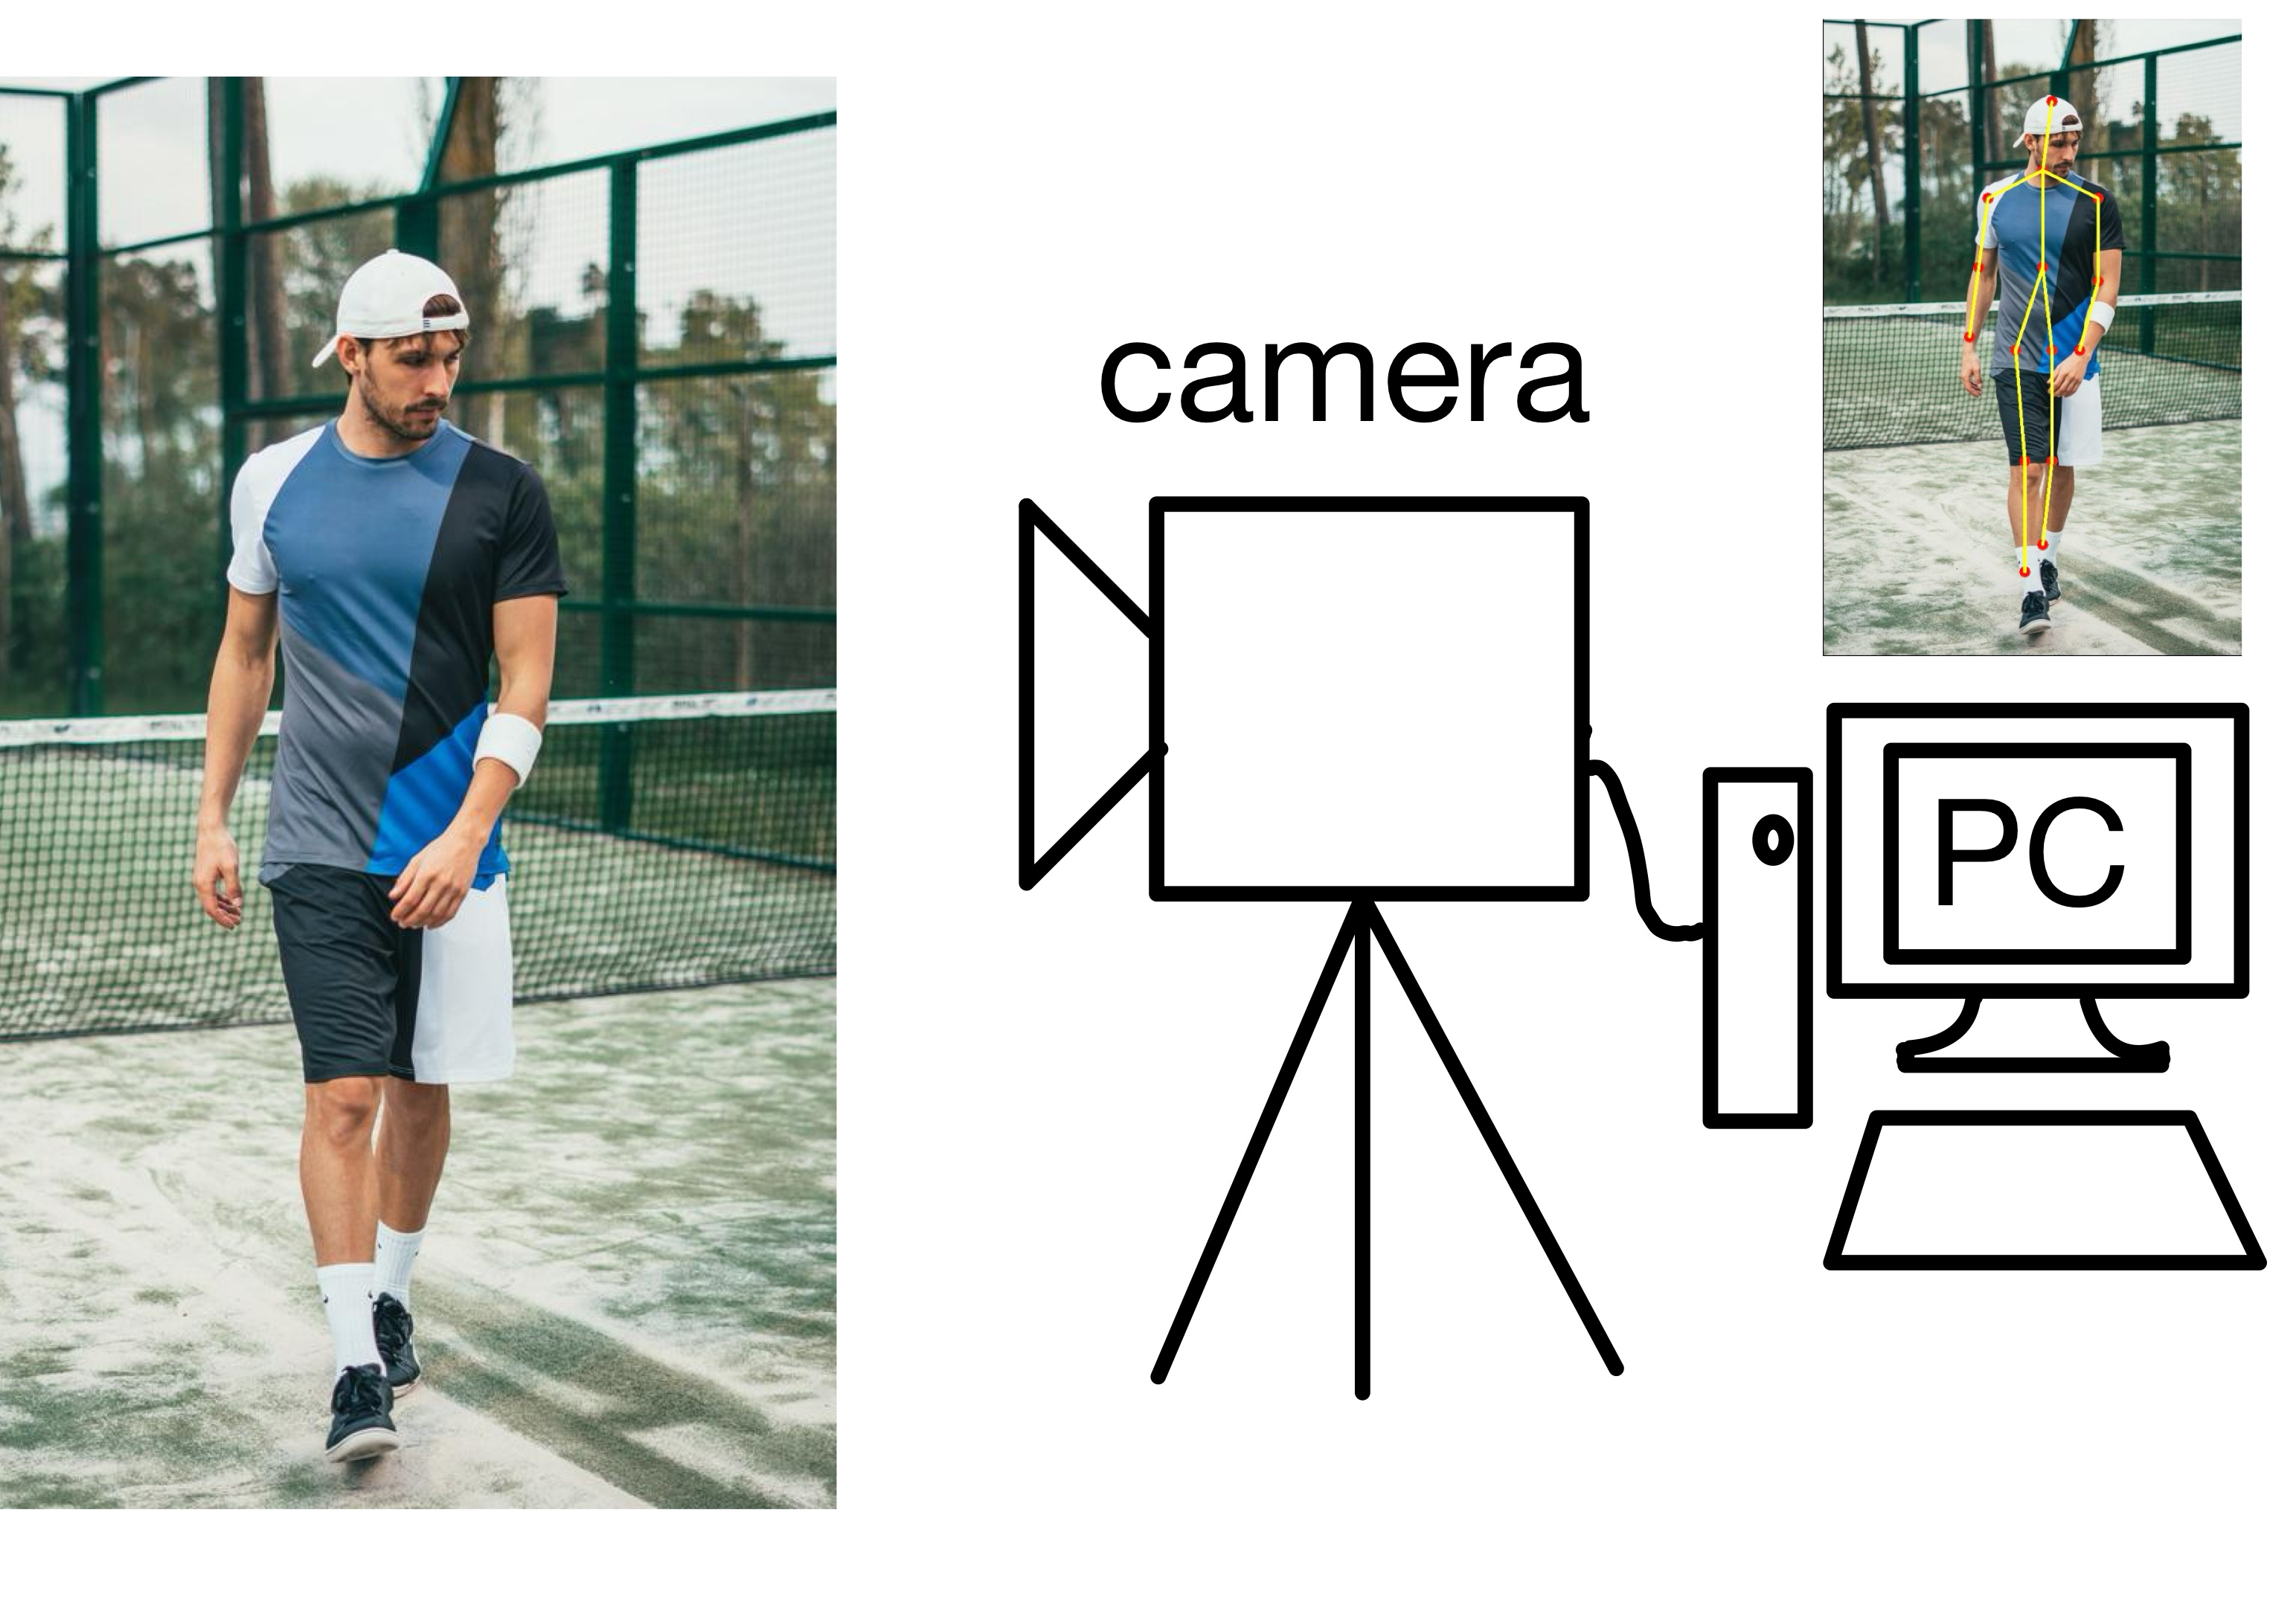
\includegraphics[width=6cm]{img/image_3D.jpg}
  \caption{画像処理による骨格推定の様子}
  \label{image_3D}
\end{figure}

カラー画像を入力としてGoogleが提供するオープンソースの機械学習ライブラリMediaPipe Poseを用いることで図\ref{RGB}に示す33個の関節の三次元骨格情報取得できる,

カラー画像と深度情報を入力として3DiVi Incが提供するライブラリNuitrackを用いることで図\ref{RGBD}に示す19個の関節の三次元骨格情報が取得できる.
% \subsection{RGBカメラ一台を用いた三次元骨格推定}\label{RGB_sec}
% 画像入力機器としてRGBDカメラであるRealSense D415を使用し,カラー画像を入力として図\ref{RGB}に示す33個の関節が取得できる,Googleが提供するオープンソースの機械学習ライブラリMediaPipe Poseで三次元計測を行う.

% \subsection{RGBDカメラで行う三次元骨格推定}\label{RGBD_sec}
% 画像入力機器としてRGBDカメラであるRealSense D415を使用し,カラー画像と深度情報を入力として図\ref{RGBD}に示す19個の関節が取得できる,3DiVi Incが提供するNuitrackで三次元計測を行う.

\subsection{慣性式モーションキャプチャの三次元骨格推定}\label{motion}
慣性式モーションキャプチャとしてmocopiを用いる.mocopiは市販のモーションキャプチャデバイスで両手,両足,頭,腰の計6ヶ所に小型センサを装着してリアルタイムに三次元計測を行うことができる.
6つの小型センサで計測しているため肘や膝などの関節部の屈曲を正確に表現することはできないが,mocopiのセンサはそれぞれ3つの自由度を持つ角度センサと加速度センサで計測しており,
機械学習を用いることで図\ref{mocopi}に示すような肘や膝などの関節部を含めた27個の関節位置を推定している.
取得するモーションデータのフレームレートは60\,fpsとする.
\begin{figure*}[t]
  \begin{tabular}{ccc}
    \begin{minipage}[]{0.3\hsize}
      \centering
      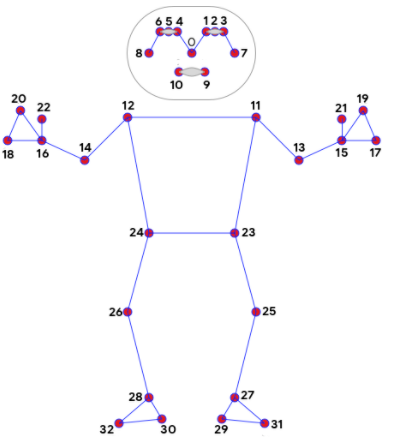
\includegraphics[height=45mm]{img/media.png}
      \subcaption{MediaPipe Poseで取得できる関節位置}
      \label{RGB}
    \end{minipage}
    \hspace{0.03\columnwidth} % ここで隙間作成
    \begin{minipage}[]{0.3\hsize}
      \centering
      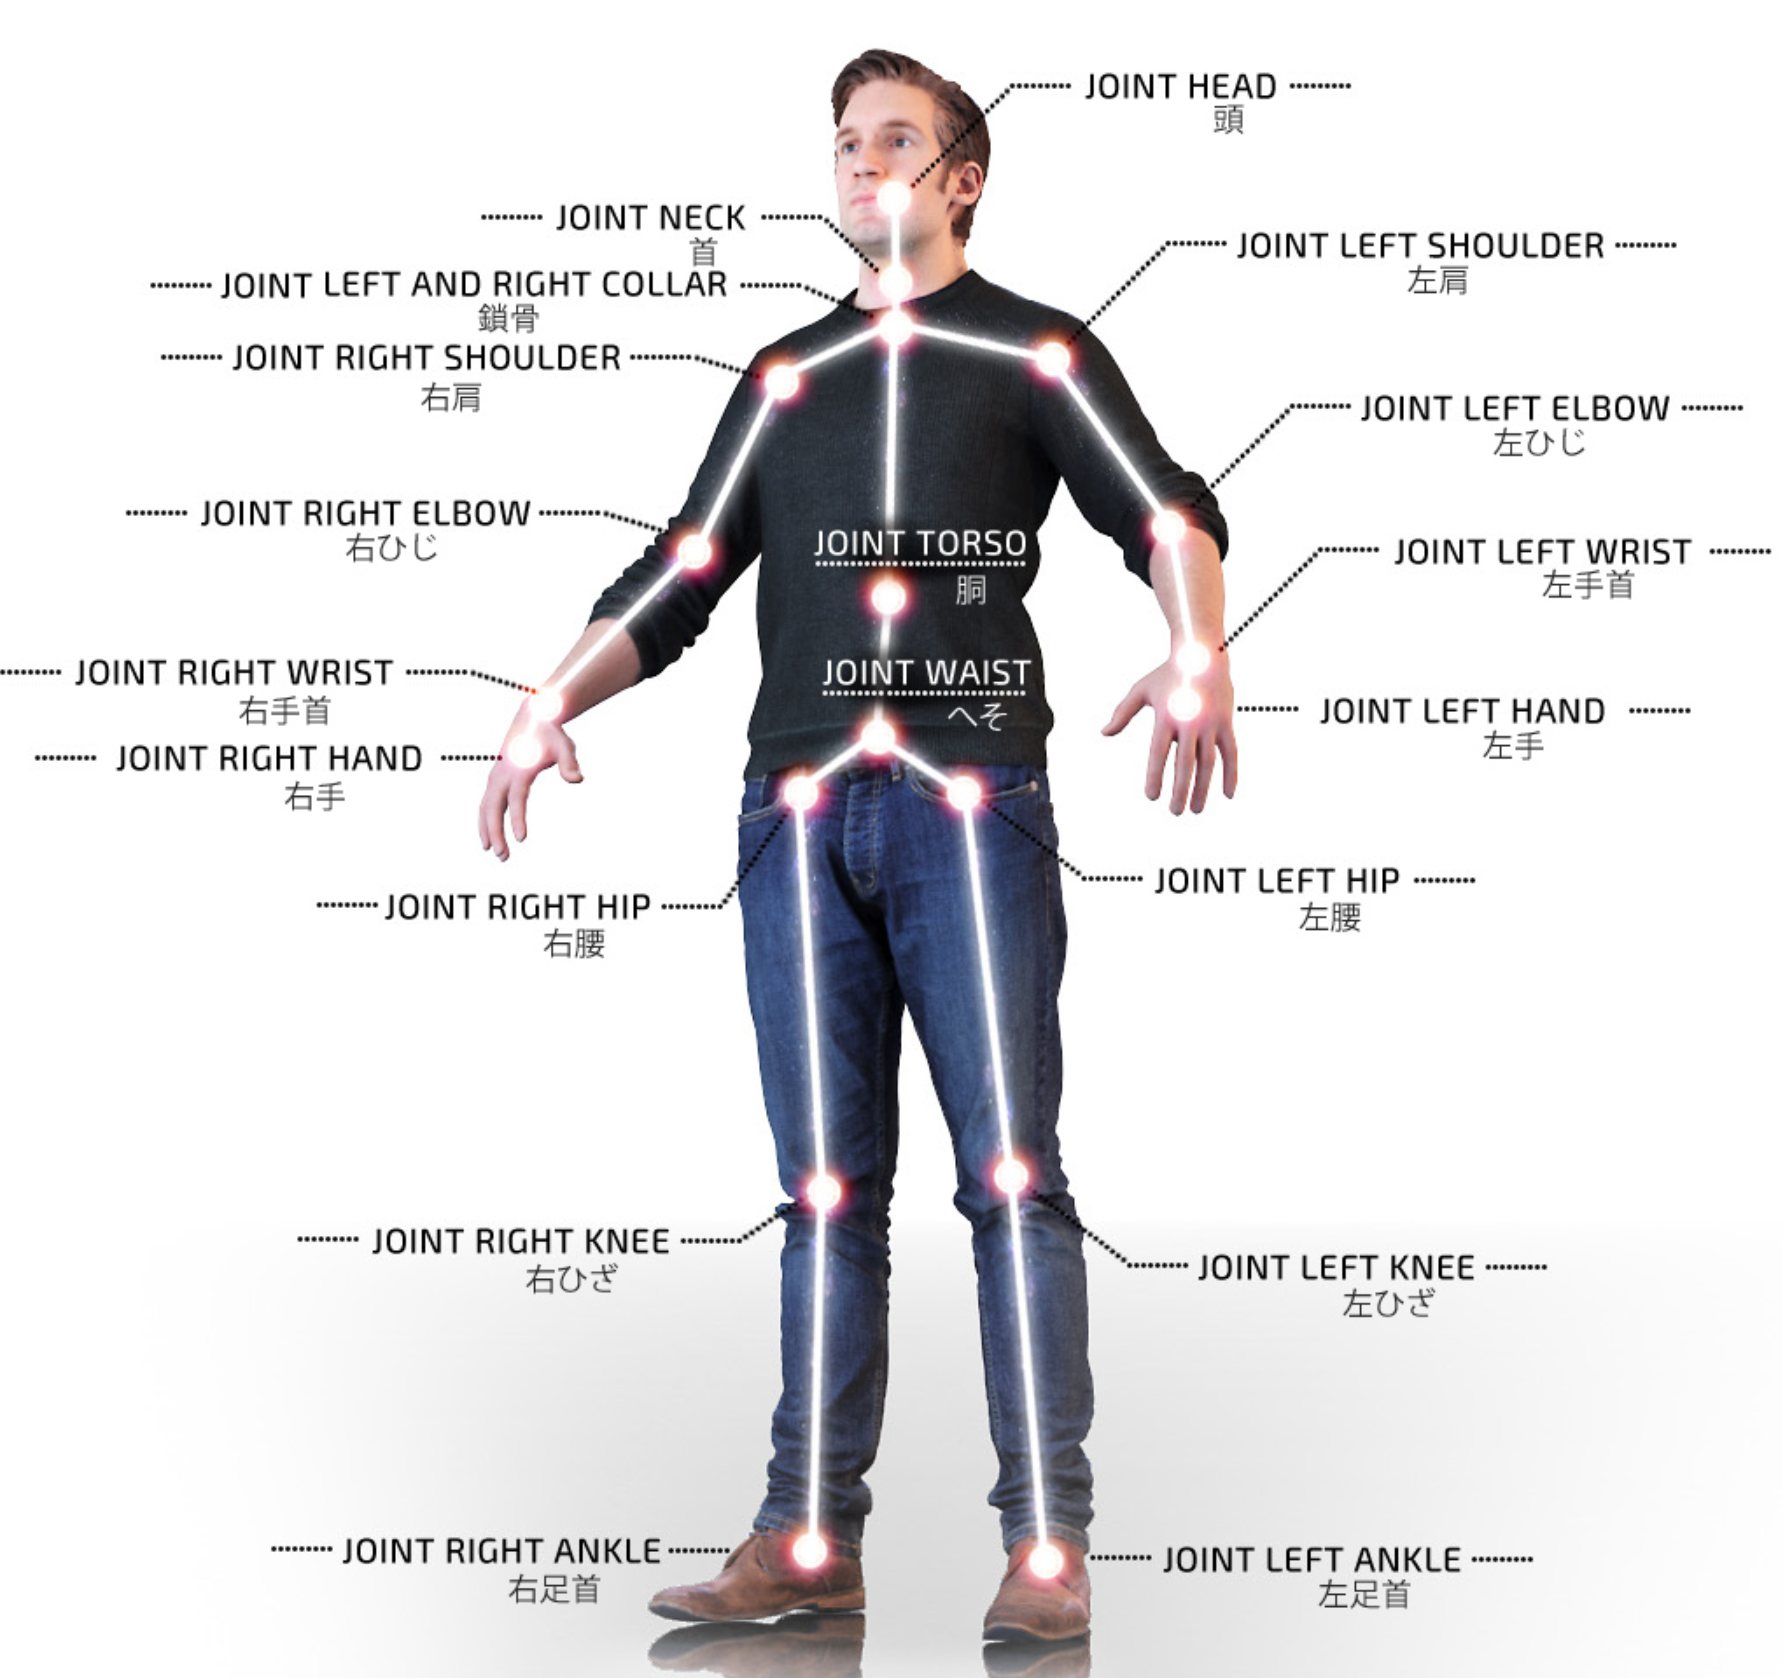
\includegraphics[height=45mm]{img/nuitrack.png}
      \subcaption{Nuitrackで取得できる関節位置}
      \label{RGBD}
    \end{minipage}
    \hspace{0.03\columnwidth} % ここで隙間作成
    \begin{minipage}[]{0.3\hsize}
      \centering
      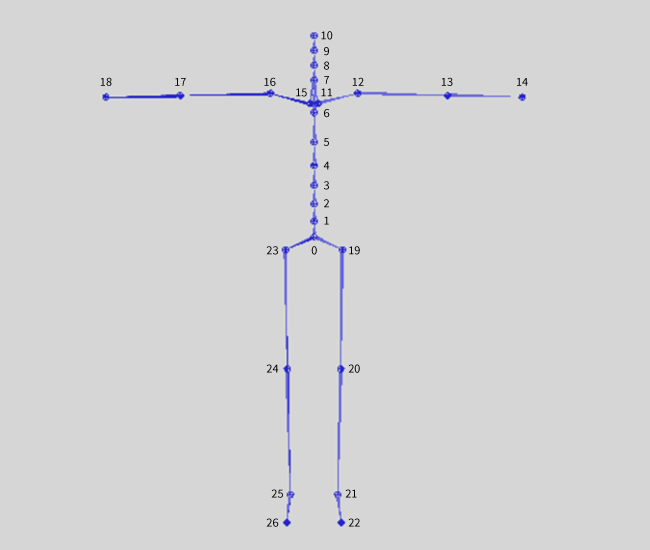
\includegraphics[height=45mm]{img/TechSpec_02.png}
      \subcaption{mocopiで取得できる関節位置}
      \label{mocopi}
    \end{minipage}
  \end{tabular}
  \caption{取得できる骨格}
  \label{sokutei}
\end{figure*}
\subsection{キャリブレーション}
全身運動を計測する前に,まず両腕を水平に上げるポーズをする.水平に上げた両手首の距離を元にスケールを合わせる.
また,へその位置を原点として,頭に向かう方向をy軸,右手から左手に向かう方向をx軸,これらに軸の直行する方向をz軸として定めた座標系に統一する.

次に両手を伸ばしたまま胸の前で合わせるポーズをする.手が合わさっている時,両手首が最接近しているので,各骨格情報の座標が最も近づいたフレームを合わせることで時間遅れを修正する.
% 計測方法により,座標系やスケール,時間遅れが異なるので同期が必要である.
% 座標系やスケール,処理により発生した時間遅れを統一するためのキャリブレーションを行う必要がある.
% キャリブレーションの方法として計測前に両腕を水平に広げ,その後腕を伸ばしたまま両手を胸の前で合わせるポーズを取る.

% 1つ目の両腕を水平に上げるポーズを元に座標系とスケールのキャリブレーションを行う.
% 水平に上げた両手首の距離を元にスケールを合わせる.
% また,へその位置を原点として,頭に向かう方向をy軸,右手から左手に向かう方向をx軸,これらの軸と直交する方向をz軸として座標系を定める.

% 2つ目の両手を伸ばしたまま胸の前で合わせるポーズでは,両手首が最接近していることを利用する.各骨格情報の両手首の座標が最も近づいたフレームを合わせることで時間遅れを修正する.
\section{研究結果}
\subsection{実験方法}
% 全身運動をしている人物一人に対して計測を行い,mocopiのセンサの位置に当たる両手,両足,頭,腰の計6ヶ所に関して,画像処理を用いた三次元骨格推定で得られた座標との誤差を比較することで精度を評価する.
全身運動をしている人物一人に対して計測を行い,計測値を人体に当てはめたときに破綻していないか,肘や膝の関節部分が正しく計測されているか,オクルージョンが起こった場合どの程度精度が落ちるのかを比較する.
計測をする前に,キャリブレーションに必要なポーズを行い,動作が緩やかでオクルージョンなし,動作が急でオクルージョンなし,動作が緩やかでオクルージョンあり,動作が急でオクルージョンありの4種類の運動を行う.
\subsection{解析結果}
今回,キャリブレーション時の右手の座標結果をxz平面に並べた結果を図\ref{1_media},\ref{1_mocopi}に示す.
\begin{figure}[h]
  \centering
  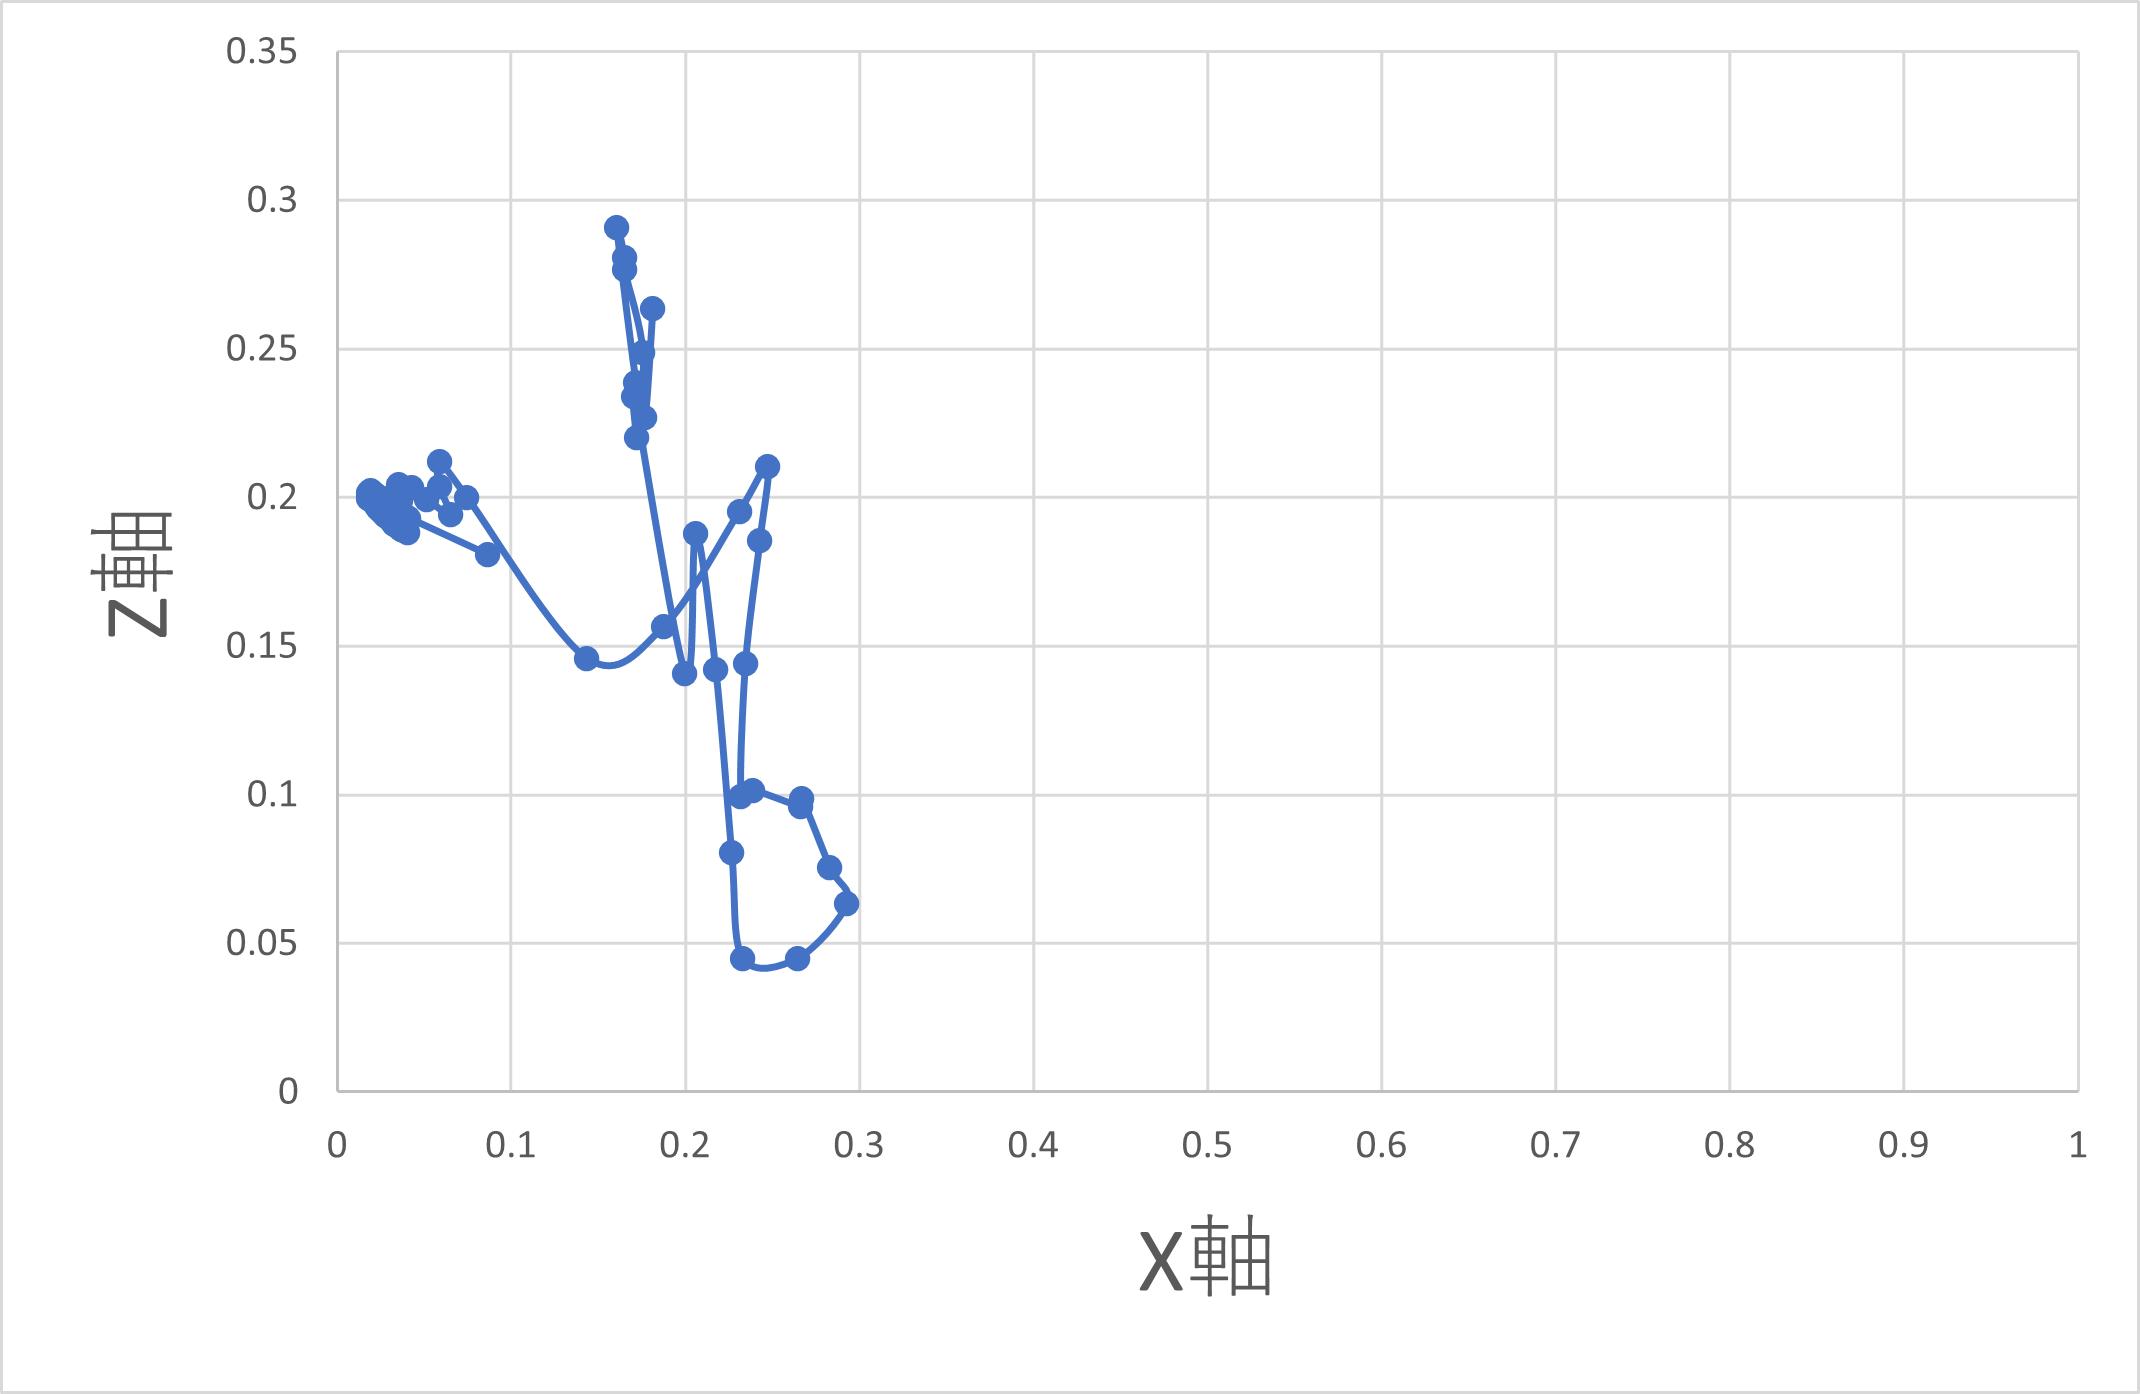
\includegraphics[width=6cm]{img/1_media.png}
  \caption{RGB画像による骨格推定データ}
  \label{1_media}
\end{figure}

\begin{figure}[h]
  \centering
  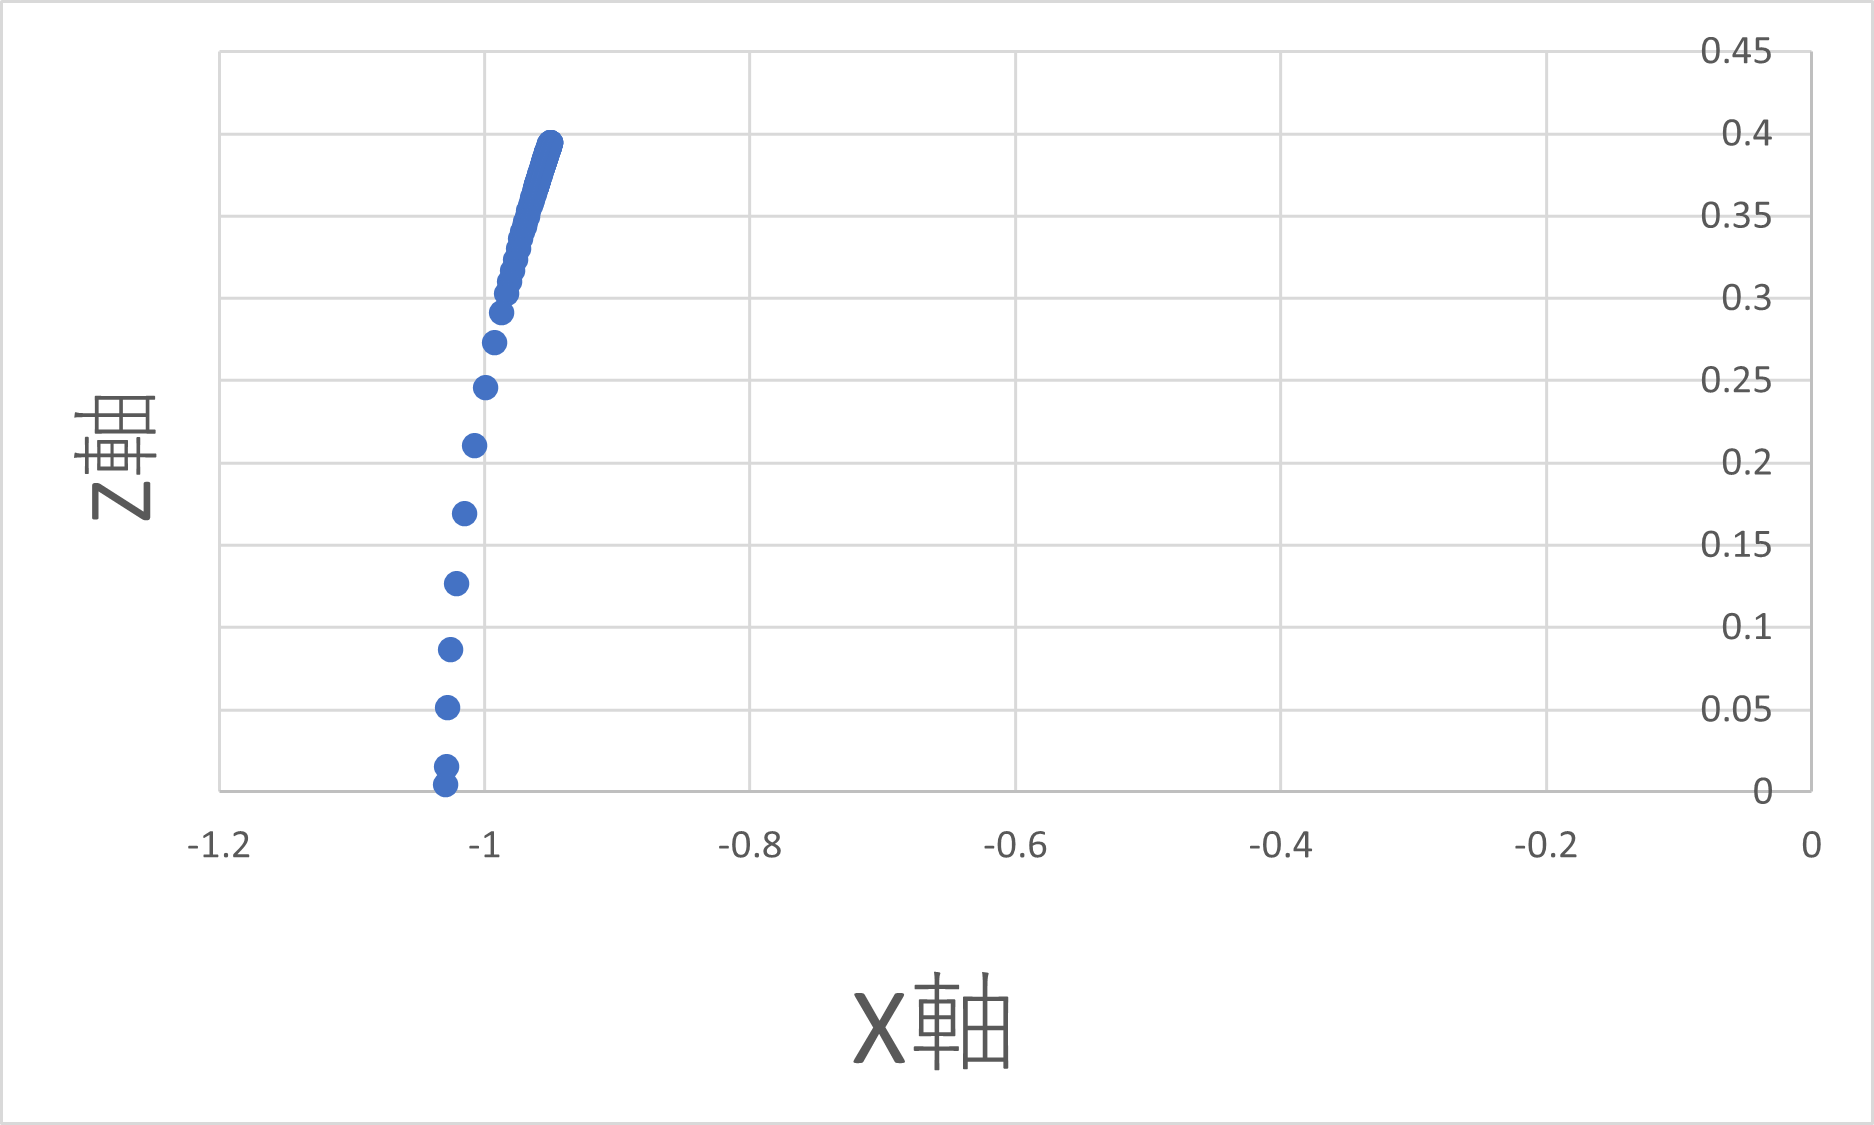
\includegraphics[width=6cm]{img/1_mocopi.png}
  \caption{慣性式モーションキャプチャによる骨格推定データ}
  \label{1_mocopi}
\end{figure}

このような人体の恒常性があるのか怪しい結果になってしまった.
このような結果になった原因として,キャリブレーションに用いた計測ポーズがキャリブレーションの方法と相性が悪い可能性や誤差を含みやすいものだった可能性が挙げられる.
\section{まとめ}
RGBDによる方法では現在問題の修正中であるがRGBDによる方法を用いることで.正しく測定できるのではないかと考えられる.
\begin{thebibliography}{99}
  \small{
    \bibitem{turugi}{
      剱 一輝,``柔道競技の3Dアーカイブ化'',令和4年度長岡高専専攻科論文,2023.
    }
    \bibitem{mediapipe}{
      Google,``mediapipe'',\\
      \url{https://developers.google.com/mediapipe}
    }




  }
\end{thebibliography}
\rightline{URLは2023年10月4日にアクセス}
\end{document}